\documentclass[]{article}
\usepackage{amsmath}
\usepackage{tikz}
\usetikzlibrary{graphs,automata}
\title{Document}
\begin{document}
\section*{\textbf{\textit{\underline{abcdefg this is my text entry}}}}

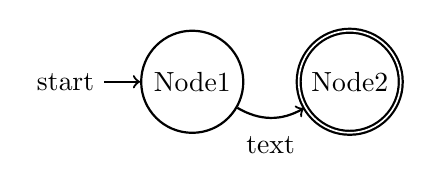
\begin{tikzpicture}[node distance={2cm}, thick, state/.style = {draw, circle}]
\node[state,initial left] (Node1) {Node1};
\node[state,accepting] (Node2) [right of=Node1] {Node2};
\path[->] (Node1) edge[bend right = 30] node[below = 0.1cm] {text} (Node2);
\end{tikzpicture}

\begin{center}
\begin{tabular}{|l|c|c|c|}
\hline
&\textbf{T1}&\textbf{T2}&\textbf{T3}\\
\hline
\textbf{L1}&a&abc&c\\
\hline
\textbf{L2}&a&b&c\\
\hline
\textbf{L3}&a&b&c\\
\hline
\end{tabular}
\end{center}

\[\begin{bmatrix}
2.0 & 2.54 & -5.0\\
3.4 & 4.4 & 5.0\\
5.0 ^ { 42.0 + ( x ) } &  \log( 5.0 ) & a \cdot ( 2.0 )\\
\end{bmatrix}\]
\end{document}
